\documentclass{beamer}
\usetheme{AnnArbor}
\usecolortheme{beaver}
\usepackage{graphicx}
\graphicspath{{images/}}
\usepackage[T1]{fontenc}
\usepackage[utf8x]{inputenc}
\usepackage[french]{babel}
\usepackage{subcaption}
\usepackage{listings} % package pour insérer les codes
\usepackage{xcolor}
\definecolor{codegreen}{rgb}{0,0.6,0} % Définir les couleurs pour les codes
\lstset{frame=tb,
  language=Java,
  aboveskip=3mm,
  belowskip=3mm,
  showstringspaces=false,
  columns=flexible,
  basicstyle={\small\ttfamily},
  numbers=none,
  numberstyle=\tiny\color{gray},
  keywordstyle=\color{blue},
  commentstyle=\color{codegreen},
  stringstyle=\color{black},
  breaklines=true,
  breakatwhitespace=true,
  tabsize=3
}

\usepackage{mathtools} % Pour les symbols mathématiques

\title[Soutenance de fin d'études]{Automatisation de Test fonctionnel et de Test Non-régression}

\author{Qilin ZHANG}
\institute{Sorbonne Université - Master 2 Informatique STL Alternance}
\date{5 Septembre 2019}
\subject{presentation}

% Table des matières à chaque début de section
\AtBeginSubsection[]
{
  \begin{frame}
    \frametitle{Plan}
    \tableofcontents[currentsection, currentsubsection]
  \end{frame}
}
\begin{document}
    % page de titre
    \begin{frame}
        \titlegraphic{
            
\includegraphics[width=2cm]{Logo_officiel_Sorbonne_University}\hspace*{1.75cm}~%
            
\includegraphics[width=2cm]{SAP_R_grad}
        }
        
        \titlepage
        \footnotesize Tuteur D'entreprise: Camilla CHRISTIANSEN, Sébastien COUDRAY \\
Tuteur universitaire: Emmanuel CHAILLOUX, Binh-Minh BUI-XUAN
    \end{frame}
    
    % Logo 
    \logo{
            
\includegraphics[height=0.5cm]{Logo_officiel_Sorbonne_University}
            
\includegraphics[height=0.5cm]{SAP_R_grad}
        }
        
    % plan
    \begin{frame}
        \frametitle{Plan}
        \tableofcontents
    \end{frame}
    
    \section{Présentation d'organisation d'accueil}
        \subsection{Présentation d'entreprise - SAP}
        
        %%%%%% Frame 1 %%%%%%
        \begin{frame}
            \begin{block} {SAP Histoire}
                SAP SE (Systems, Applications \& Products in Data Processing), fondé par 5 anciens IBM employés en 1972
            \end{block}
            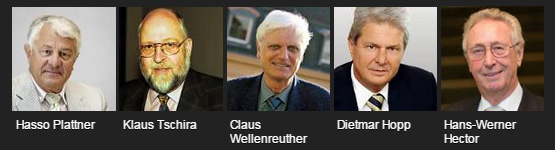
\includegraphics[width=5cm,]{sap_founders.jpg}
            \begin{block}{SAP Information}
            \begin{itemize}
                \item 1\textsuperscript{er} éditeur de logiciels en Europe et 4\textsuperscript{ème} dans le monde
                \item Le plus grand fournisseur mondial de logiciels d’application d’entreprise
                \item Entreprise internationale : Plus de 98000 employés au tour du monde dans plus de 147 pays, plus de 437000 clients dans plus de 180 pays.
                
            \end{itemize}
            \end{block}
            
            \begin{block}{SAP France}
                \begin{columns}
                \column{0.85\textwidth}
                \begin{itemize}
                    \item Locale: \textbf{Tour SAP} 35 rue d’Alsace, 92300 Levallois-Perret
                    \item Présente plus de 1500 de salariés en temps plein.
                \end{itemize}
                
                \column{0.2\textwidth}
                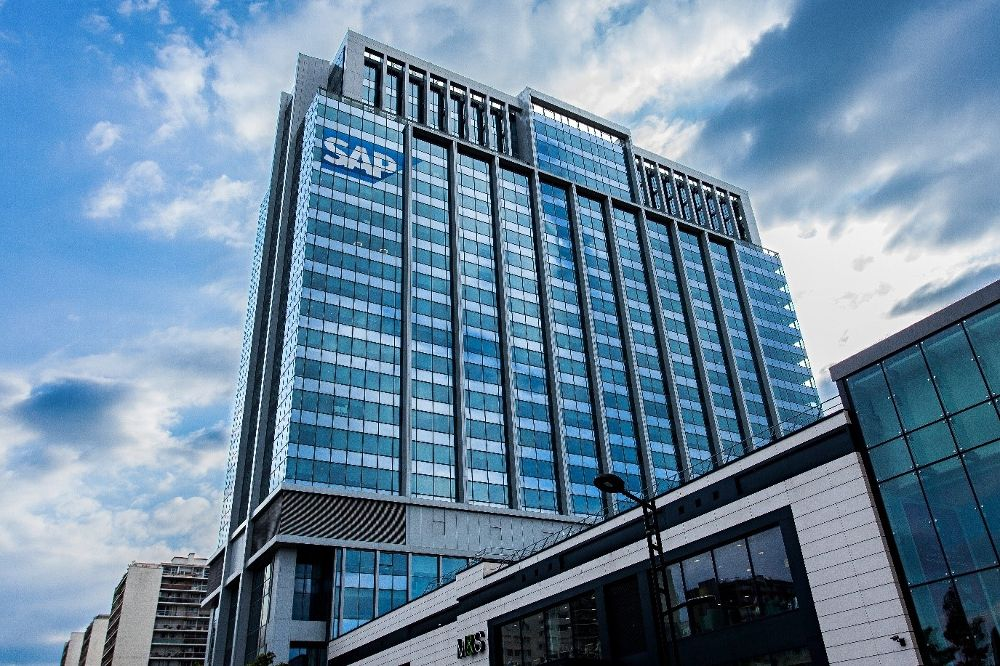
\includegraphics[width=\textwidth]{sap-france.jpg}
                \end{columns}
            \end{block}
            
        \end{frame}
        
        %%%%%% Frame 2 %%%%%%
        \begin{frame}
            \frametitle{SAP Produits et Slogan}
            \begin{columns}
            \column{0.7\textwidth}
                    8 Catégories des produits en globales : 
                    \begin{itemize}
                        \item ERP et coeur numérique
                        \item Gestion de la relation client et expérience client
                        \item Réseau et gestion des dépenses
                        \item Chaîne logistique digitale
                        \item RH et implication du personnel
                        \item Plateforme digitale
                        \item Outils d’analyse
                        \item Technologies intelligentes
                    \end{itemize}
            \column{0.3\textwidth}
            SAP Slogan : \\ The Best run SAP
            \flushleft
            
\includegraphics[width=\textwidth]{SAP_Best_R_grad_blk.jpg}
            \end{columns}
        \end{frame}
        
        %%%%%% Frame 3 %%%%%%
        \begin{frame}
            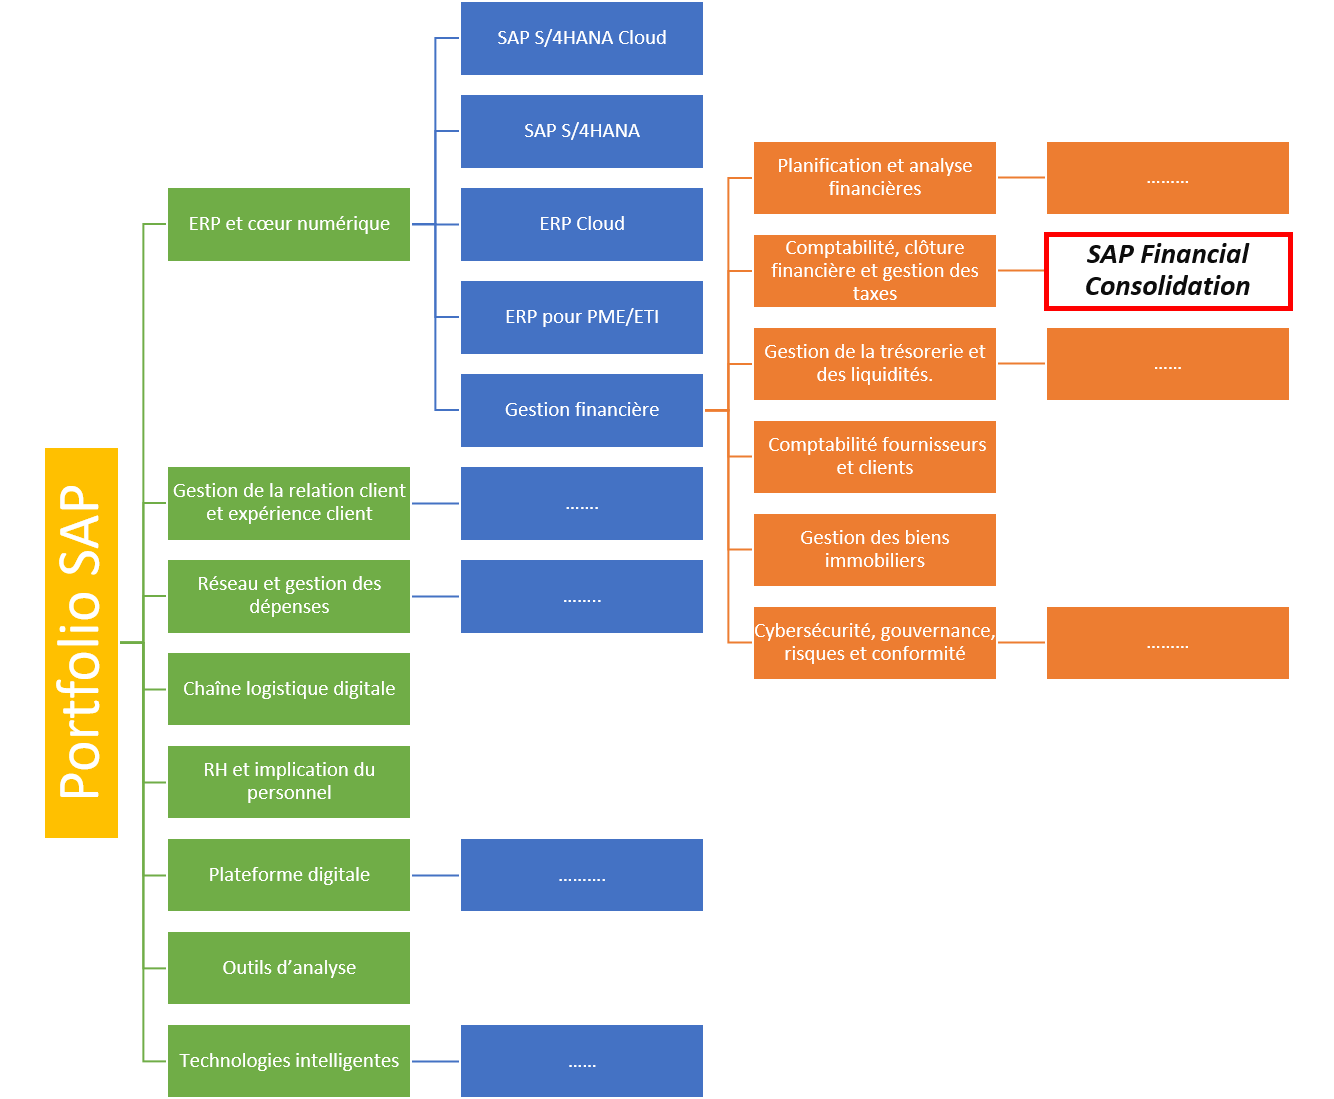
\includegraphics[height=8cm]{SAP_portfolio.png}
        \end{frame}
        
        %%%%%% Frame 4 %%%%%%
        \begin{frame}
            \frametitle{SAP Financial Consolidation}
            \begin{block}{SAP Financial Consolidation}
            \begin{itemize}
                \item \textbf{SAP Financial Consolidation}, la catégorie ERP et coeur numérique
                \item Une application de consolidation légale et de reporting de gestion développée depuis 1999.
                \item Il permet aux grandes entreprises de répondre à des exigences de consolidation complexes, de rationaliser la conformité réglementaire, d’unifier le reporting légal et de gestion et d’accélérer le processus de clôture financière global
            \end{itemize}
            
            \end{block}
        \end{frame}
        
        \begin{frame}
            \begin{columns}
                \column{0.5\textwidth}
                \begin{figure}
                    \centering
                    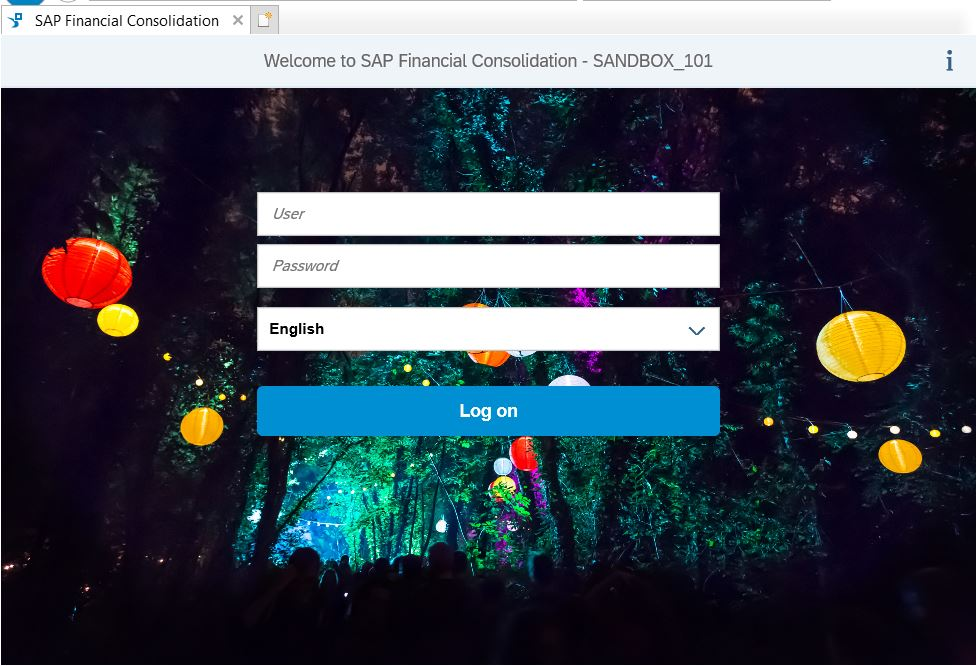
\includegraphics[width=\textwidth]{FC_pageLogin.JPG}
                    \caption{Page Login de FC}
                    \label{fig:FC_login_label}
                \end{figure}
                
                \column{0.5\textwidth}
                \begin{figure}
                    \centering
                    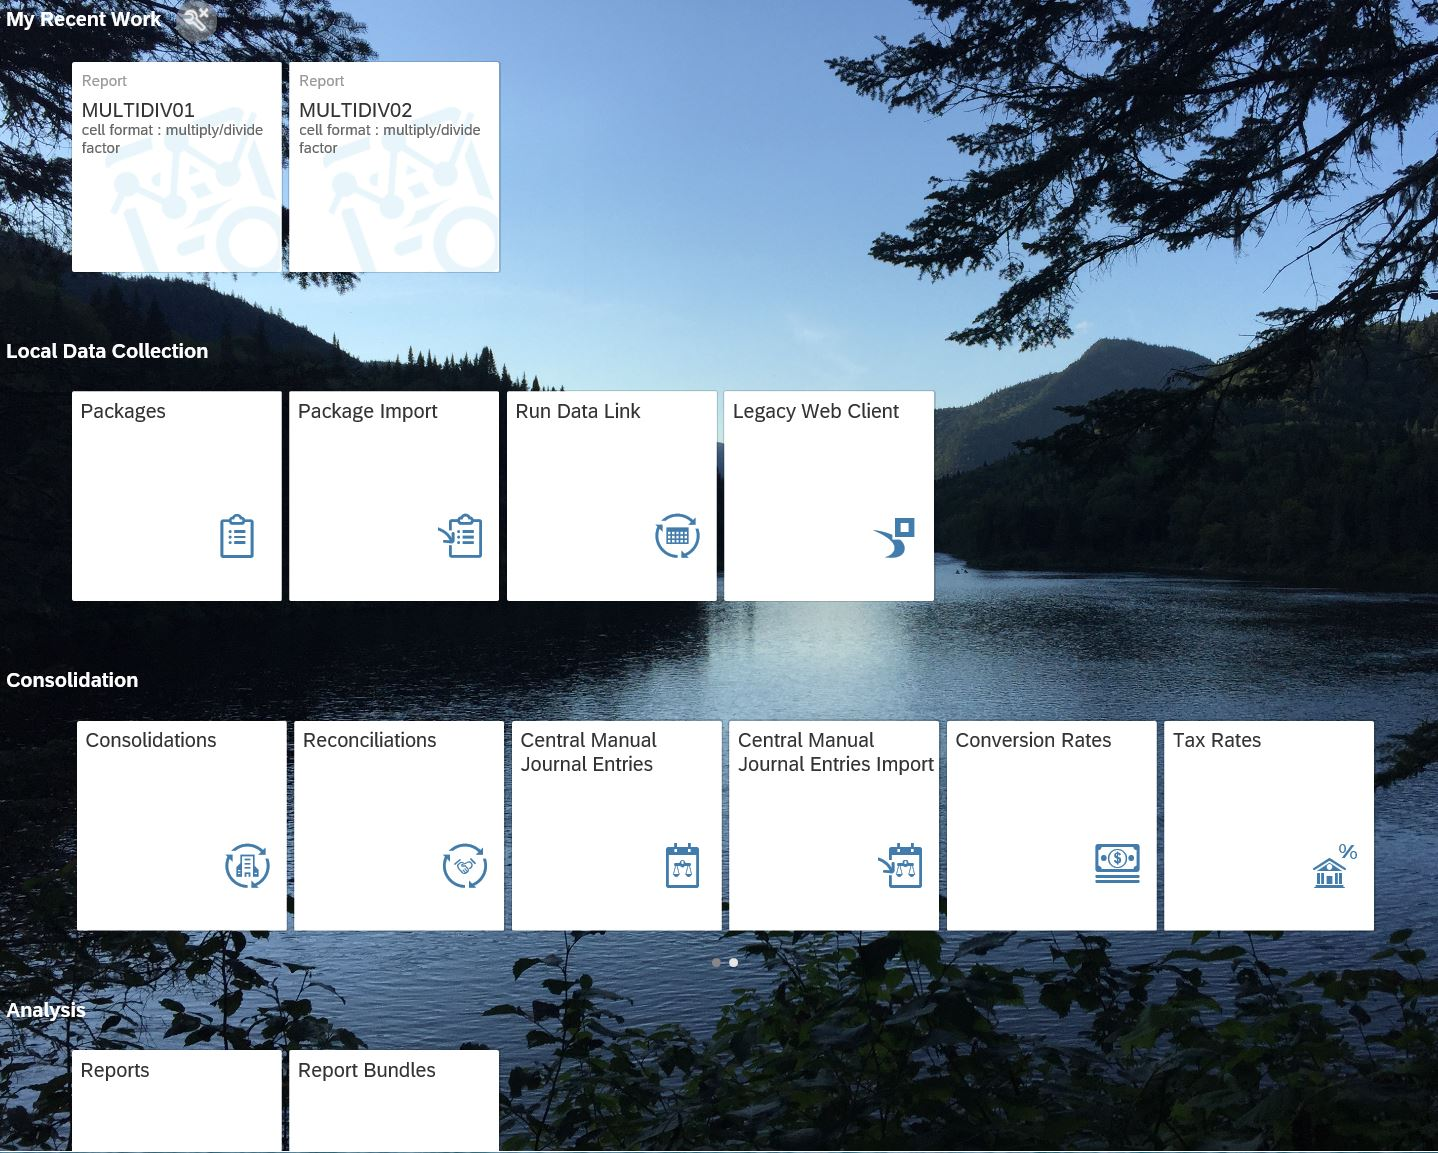
\includegraphics[width=\textwidth]{FC_Homepage.JPG}
                    \caption{Home page de FC}
                    \label{fig:FC_homepage_label}
                \end{figure}
            \end{columns}
            
        \end{frame}
        
        \subsection{Introduction d'équipe}
        %%%%%% Frame 4 %%%%%%
        \begin{frame}
        \frametitle{Organisation d'équipe et mon rôle}
            \begin{block}{Rôle et Mission}
            \begin{itemize}
                \item Apprenti Ingénieur de Qualité, intégré à l'équipe P\&I S/4HANA LoB Finance France, partie Test de sous-équipe FC
                \item Automatiser des scénarios de tests fonctionnels et de non-régression
            \end{itemize}
            
            \end{block}
            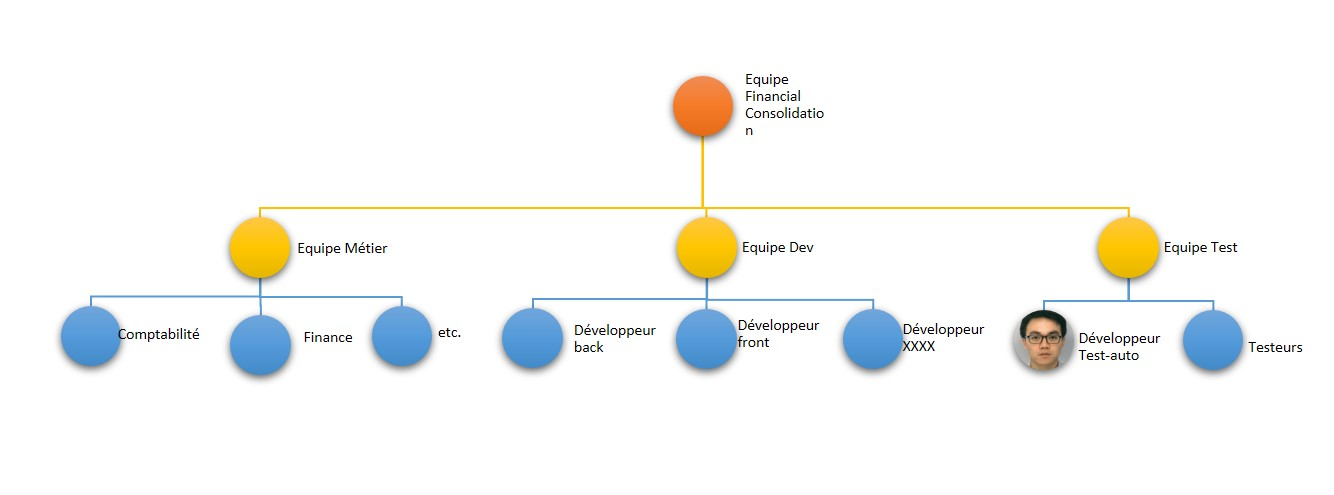
\includegraphics[width=\textwidth]{role_organisation.jpg}
        \end{frame}
        
        \begin{frame}
        \frametitle{Organisation d'équipe et mon rôle}
            \begin{block}{Rôle et Mission}
                \begin{itemize}
                    \item Equipe plus de 40 personnes, travaillent en méthode d'Agile
                \end{itemize}
            \end{block}
            \centering
            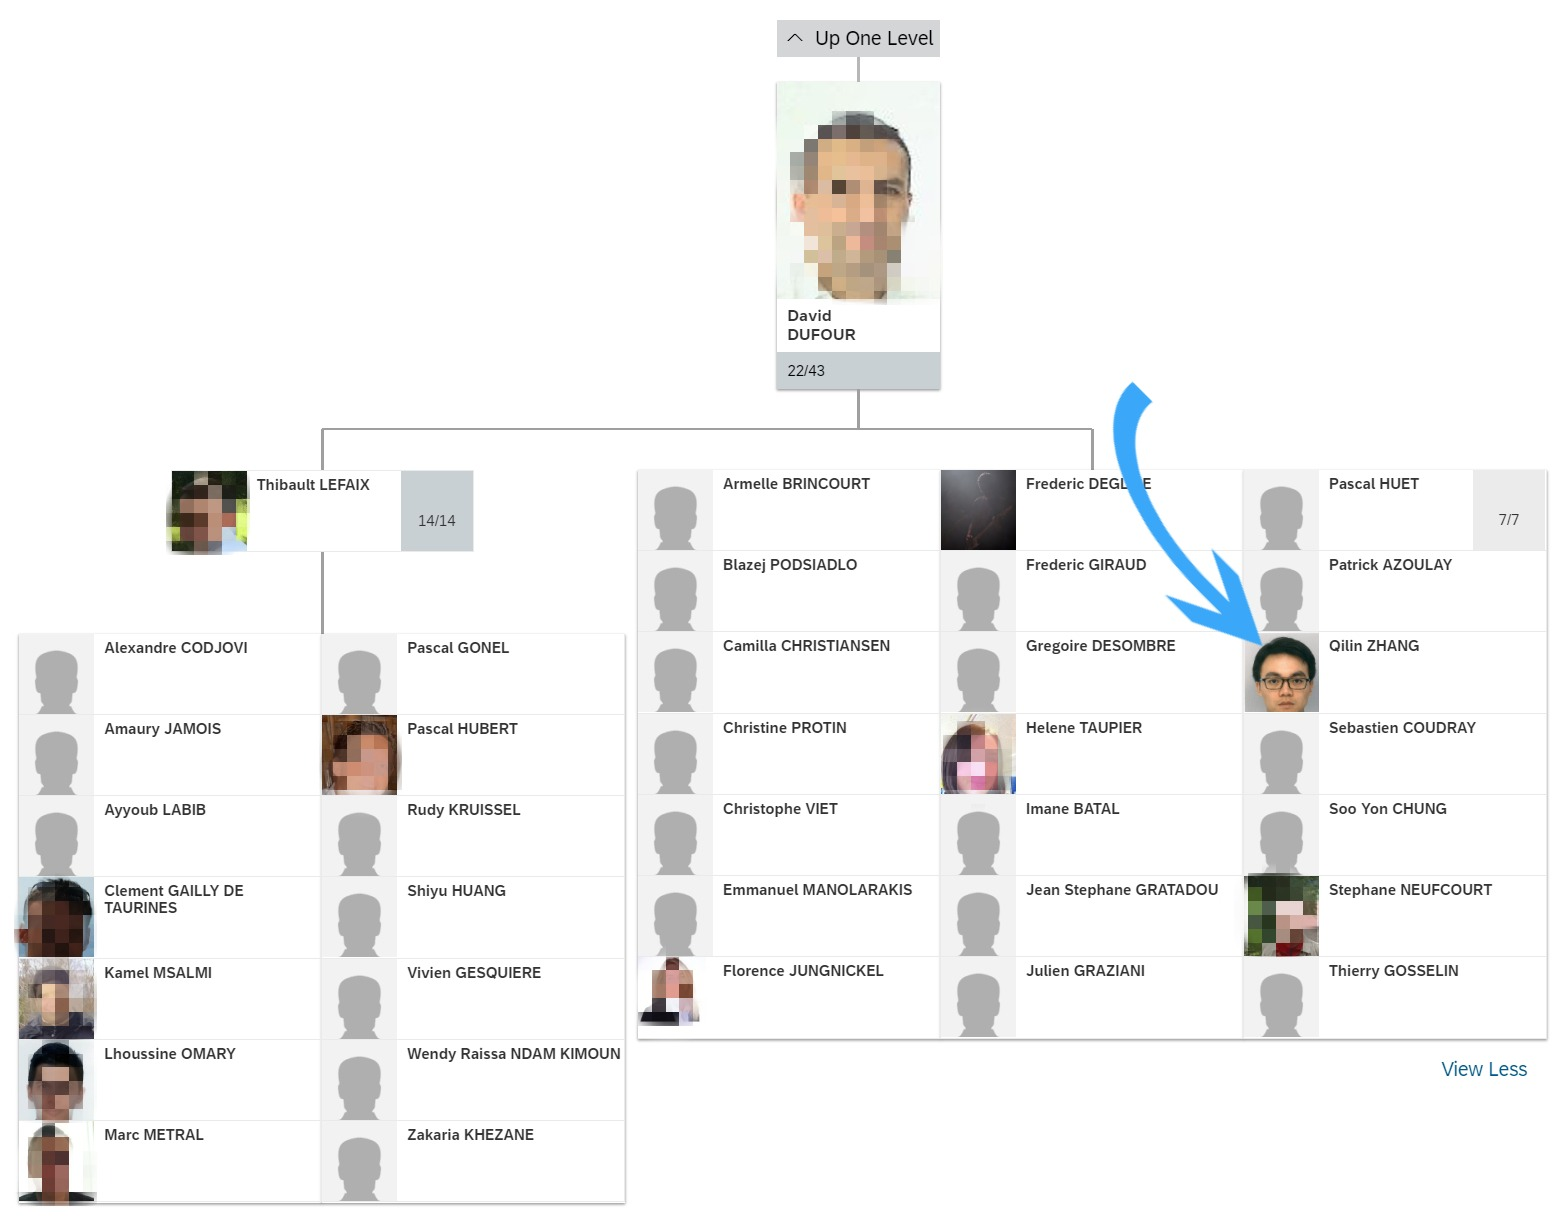
\includegraphics[width=8cm]{organisation_groupe.jpg}
        \end{frame}
        
    \section{Contexte et la problématique}
        \subsection{SAP Financial Consolidation}
        %%%%%% Frame 5 %%%%%%
        \begin{frame}
            \frametitle{Architecture de SAP Financial Consolidation}
            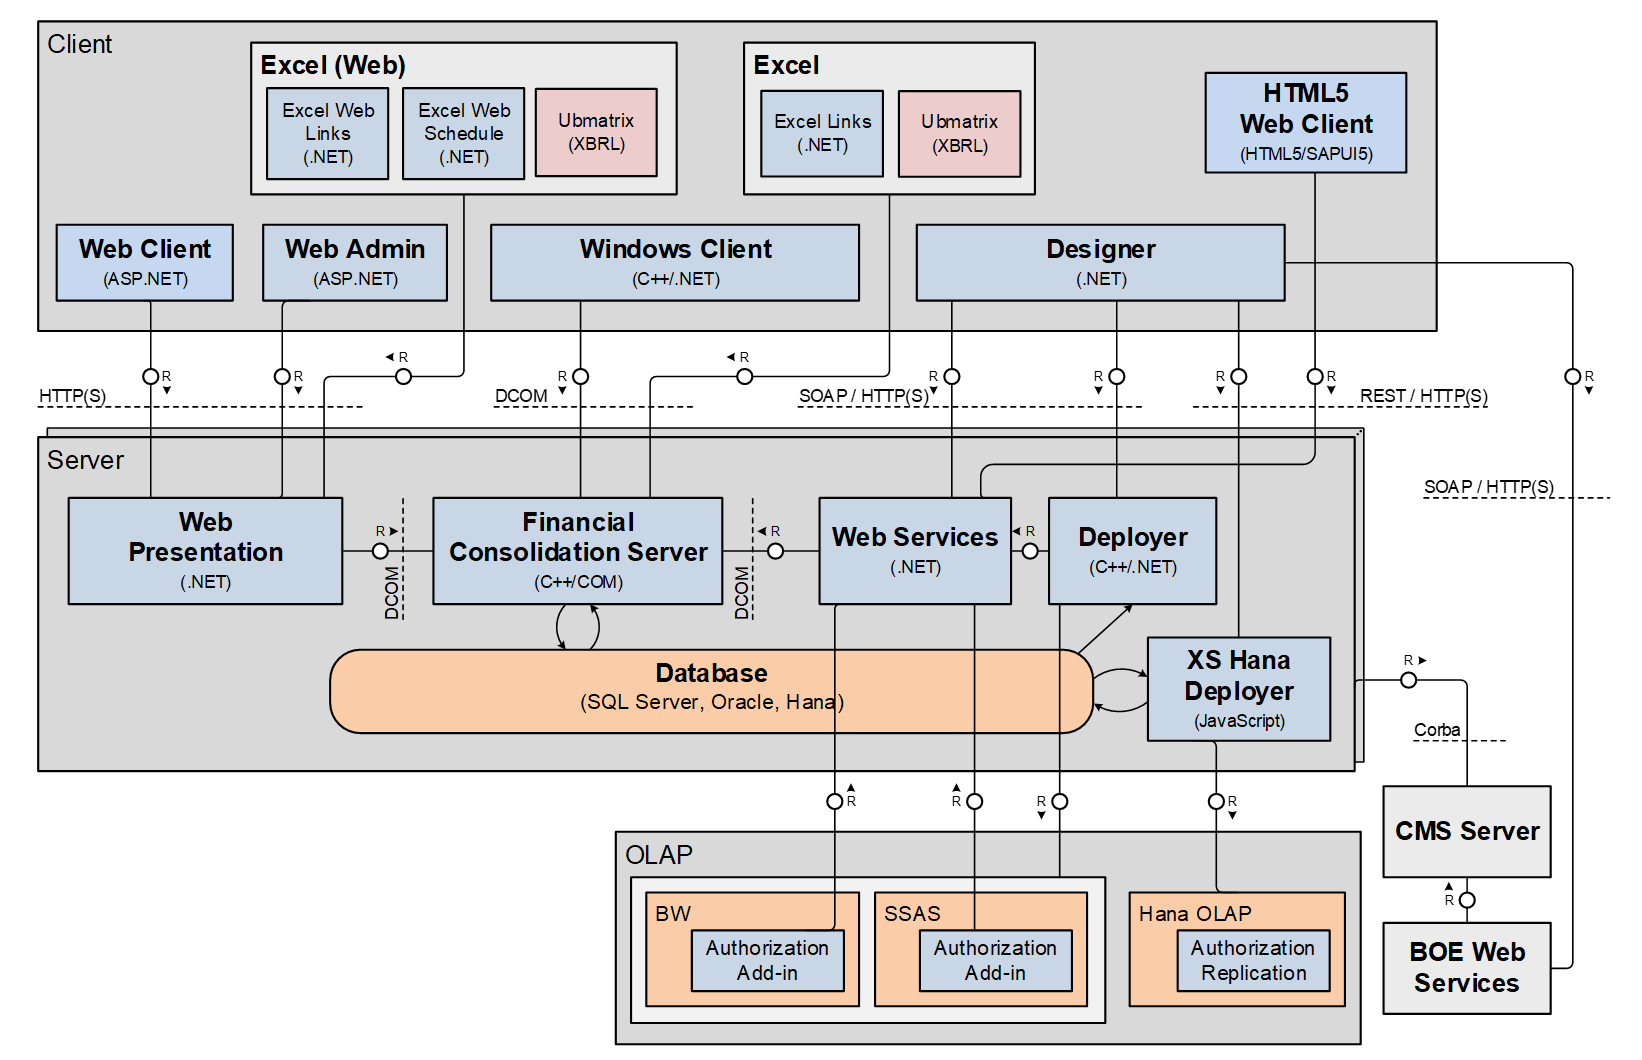
\includegraphics[width=0.84\textwidth]{FC_Globale_Architecture.png}
        \end{frame}
        
        %%%%%% Frame 6 %%%%%%
        \begin{frame}
        \frametitle{Différentes versions du client}
            \begin{description}
                \item [Client Windows Desktop :] Client installer sur Windows
                \item [Client Legacy Web :] Client version Web avant l'utilisation de HTML5
                \item [Client HTML5 Web :] Client version Web avec l'utilisation de HTML5, nouvelle UX, sortie depuis pour FC 10.1 à partir de 2015, continuer à développer les nouvelles fonctionnalités et faire les maintenances.
            \end{description}
        \end{frame}
        
        %%%%%% Frame 7 %%%%%%
        \subsection{Test régression et Test non-régression}
        \begin{frame}
            \frametitle{Le cycle de Build - Test - Release}
            \begin{columns}
                \column{0.6\textwidth}
                \centering
                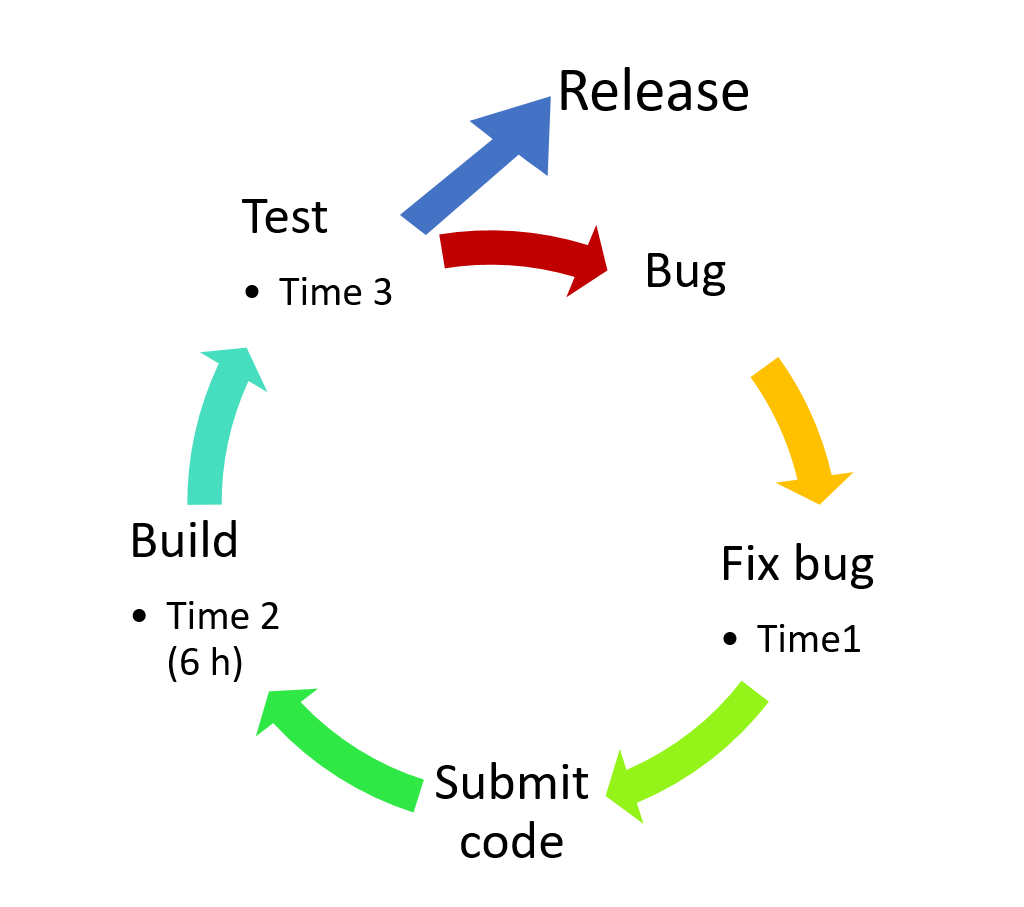
\includegraphics[width=8cm]{cycle_build_release.png}
                
                \column{0.4\textwidth}
                Différentes branches : 
                \begin{itemize}
                    \item Core: Toutes les fonctionnalités
                    \item PI : La version à tester
                    \item REL : La version livrerée directement au client
                \end{itemize}
            \end{columns}
        \end{frame}
        
        
        
        %%%%%% Frame 8 %%%%%%
        \begin{frame}
            \frametitle{Deux types de Test}
            \begin{block}{Test de régression}
                Test fonctionnel sur des nouvelles fonctionnalités ou les corrections des Bugs
            \end{block}
            
            \begin{block}{Test de non-régression}
            Pour s'assurer qu'après une modification, des défauts n'ont pas été introduits ou découverts dans des parties non modifiées.
            \end{block}
            \pause
            %\begin{alertblock}{{\LARGE{Ces deux test assurent la qualité du produit}}}
            
            %\end{alertblock}
            \centering
            \alert{{\Large{\textbf{Ces deux test assurent la qualité de produit !!!}}}}
        \end{frame}
        
        \subsection{Test d'impression}
        
        %%%%%% Frame 9 %%%%%%
        \begin{frame}
            \frametitle{Problématique de Test d'impression}
            \begin{itemize}
                \item FC contient la fonctionnalité d'impression des rapports,  le \textit{\textbf{test de non-régression}} assure la qualité de cette fonctionnalité.
                \pause
                \item Vérifie si l'impression de différente version donne le même résultat, indique la différence s'ils sont différents
            \end{itemize}
             
            \begin{figure}[H]
                \centering
                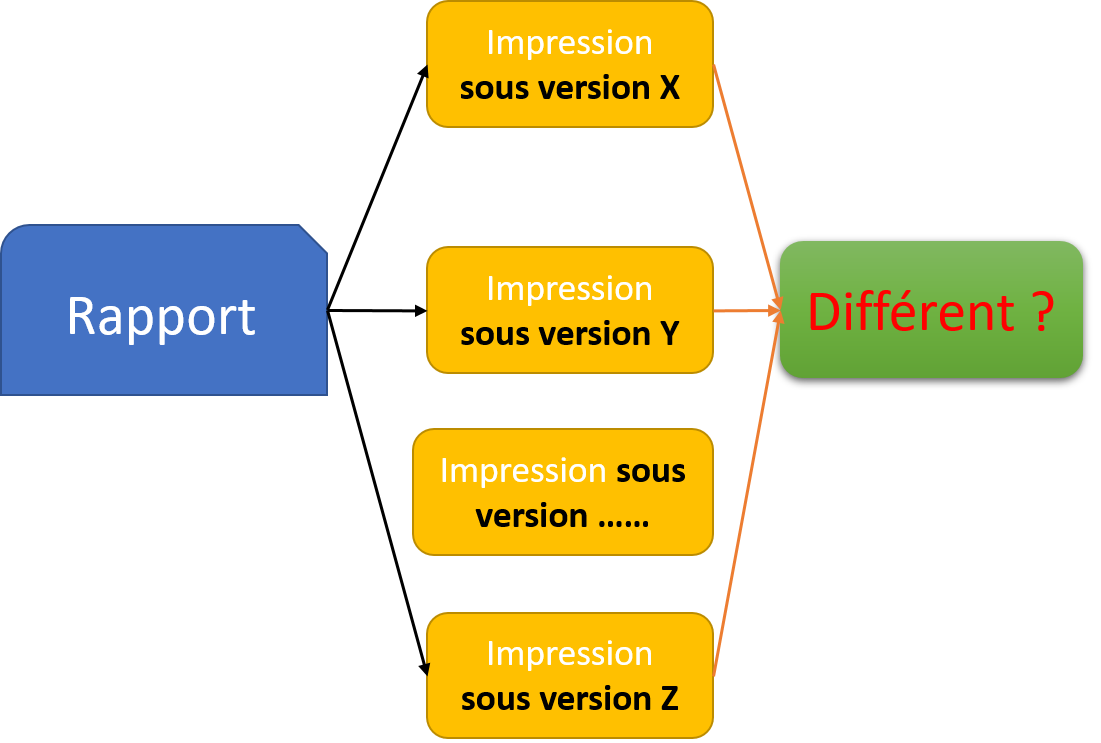
\includegraphics[width=7cm]{problematique_print.png}
                \label{fig:problem_print}
            \end{figure}
                
        \end{frame}
        
        %%%%%% Frame 10 %%%%%%
        \begin{frame}{Etat de l'art}
            \begin{block}{Etat de travail}
                \begin{itemize}
                    \item Avant mon arrive, l'équipe a fait ce test manuellement. Facile d’être fatigué faces aux scénarios répétés, perdre beaucoup de temps. 
                    \item Projet de test-auto en langage Java et plusieurs autres technologies a été développé depuis quelques années, continue à couvrir plus de fonctionnalités.
                \end{itemize}
            \end{block}
            \pause
            
            \begin{block}{Statut d'autres équipes de SAP France}
                \begin{itemize}
                    \item L'autre équipe a fait le projet de la comparaison entre deux fichier pdf pixel par pixel en Java, en utilisant une bibliothèque open source ice-pdf.
                \end{itemize}
            \end{block}
            
        \end{frame}
        
        \begin{frame}{Choix des technologies pour le Projet Test-Auto}
            \begin{block}{Silk Test, Selenium dans future}
                \begin{itemize}
                    \item \textbf{Silk Test est choisit}:
                        \begin{enumerate}
                            \item Cette technologie est déjà utilisée par l'autre équipe de SAP avant le commence de projet test-auto
                            \item Java a été de préférence du développeur pour commencer le projet.
                        \end{enumerate}
                    \item \textbf{Selenium pour le future} : Open-source, multiplateforme, plusieurs langages : Java, C\#, Perl, Python, JavaScript, Rudy, PHP, etc.
                \end{itemize}
            \end{block}
            
            \begin{block}{Comparaison par Pixel, pas de Checksum du fichier}
                \begin{itemize}
                    \item \textbf{Checksum}: Rapide, mais ne peut pas inquer la différence
                    \item \textbf{Comparaison par Pixel}: Plus difficile à programmer, mais c'est gérable, en plus, peut indiquer la différence.
                \end{itemize}
            \end{block}
            
        \end{frame}
    \section{Travaux Réalisés}
        \subsection{Architecture de Test auto}
        %%%%%% Frame 11 %%%%%%
        \begin{frame}
            \frametitle{Projet Test-Auto : Comment ça marche ?}
            \begin{enumerate}
                \item \textcolor{orange}{3} types de machines virtuelles pour business-logic : \textit{\textbf{Base de Donnée}}, \textit{\textbf{ressources de références}}, \textit{\textbf{Jenkins slave}}; \textcolor{orange}{1} machine virtuelle pour sauvegarder  les \textit{\textbf{logs}} dans une base de donnée, puis visualiser en Excel
                \item Codes sources en Java, manipulé par Perforce
                \item Un Jenkins master lancer le projet
            \end{enumerate}
        
            \centering
            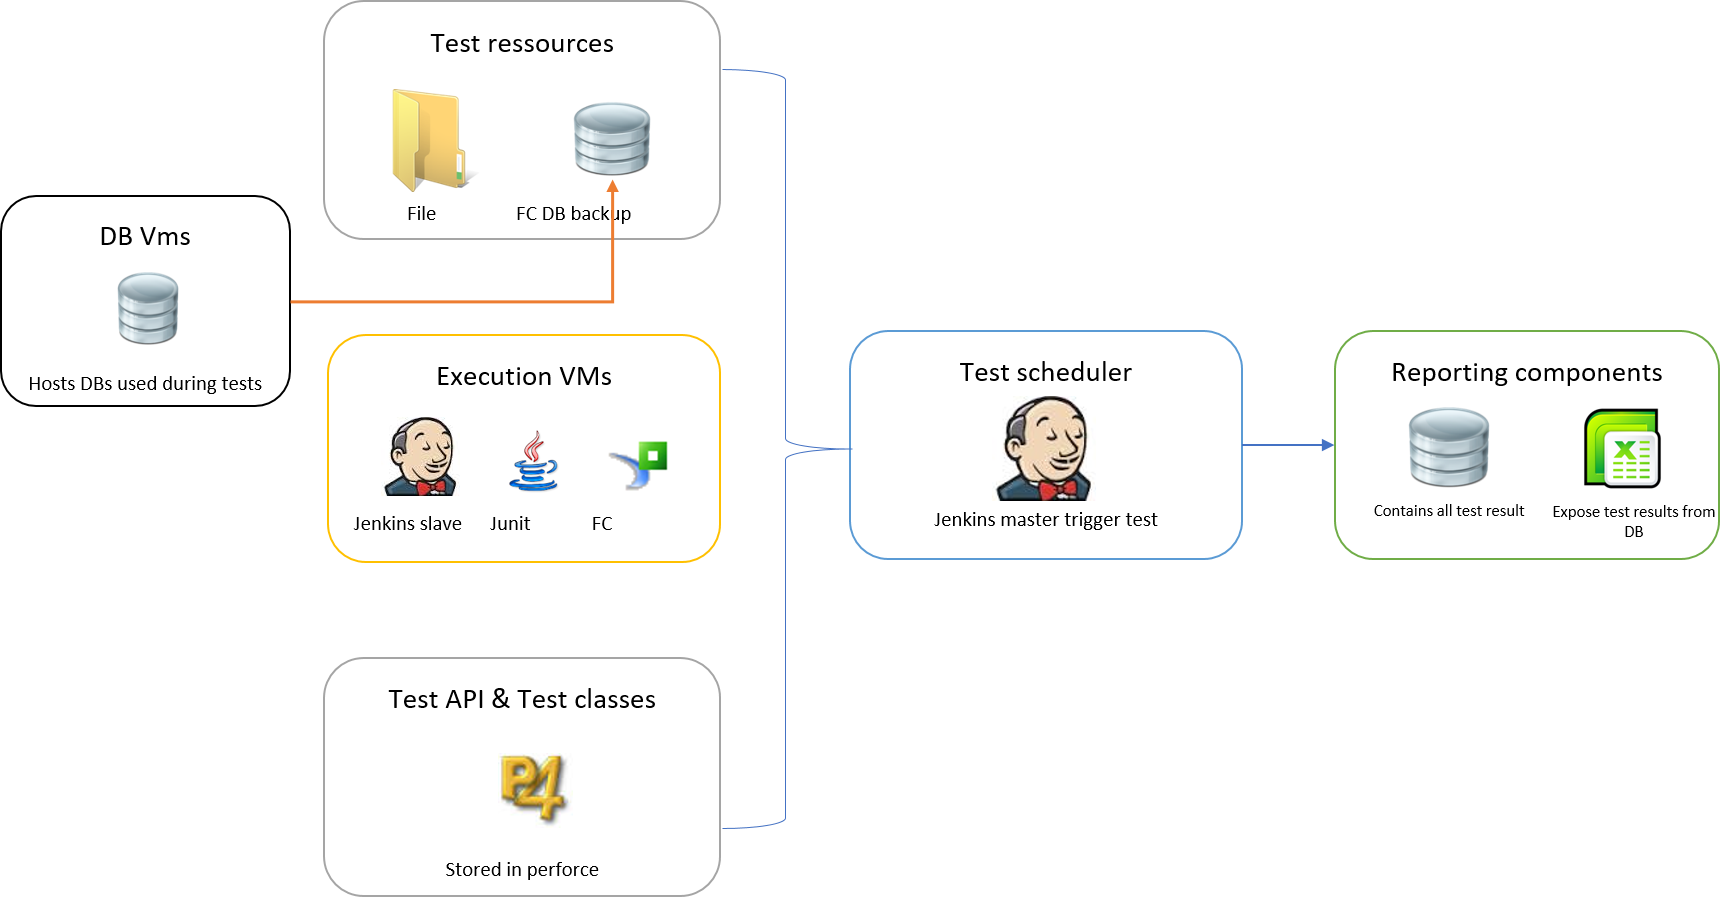
\includegraphics[width=9.5cm]{TestAuto_architecture.png}
        \end{frame}
        
        \subsection{Développements Réalisés}
        %%%%%% Frame 12 %%%%%%
        \begin{frame}
            \frametitle{1\textsuperscript{ère} tâche - Automatisation des scénarios de Test avec JUnit}
            \begin{block}{Contenus de tâche}
                \begin{itemize}
                    \item Lire et comprendre les codes existants du projet.
                    \item Programmer des tests de Junit avec langage Java, l'intègre dans projet de test-auto.
                \end{itemize}
            \end{block}
            
            \pause
            \begin{block}{Résultats}
                \begin{itemize}
                    \item Des scénarios de test bien finis et intégrés dans le projet Test-Auto
                    \item \begin{enumerate}
                        \item Bien compris l'architecture de Test-auto, comment le projet Test-auto fonctionne
                        \item Bien compris et pratiqué les technologies utilisées dans le projet : 
                            \begin{itemize}
                                \item Comment les contrôles d'application sont reconnues par XPath.
                                \item Comment SilkTest déclenchhe les navigateurs: IE, Chrome, MS Edge.
                            \end{itemize}
                    \end{enumerate}
                \end{itemize}
            \end{block}
        \end{frame}
        
        %%%%%% Frame 13 %%%%%%
        \begin{frame}
            \frametitle{2\textsuperscript{ème} tâche: Comparaison entre deux PDF}
            \begin{columns}
            \column{0.7\textwidth}
            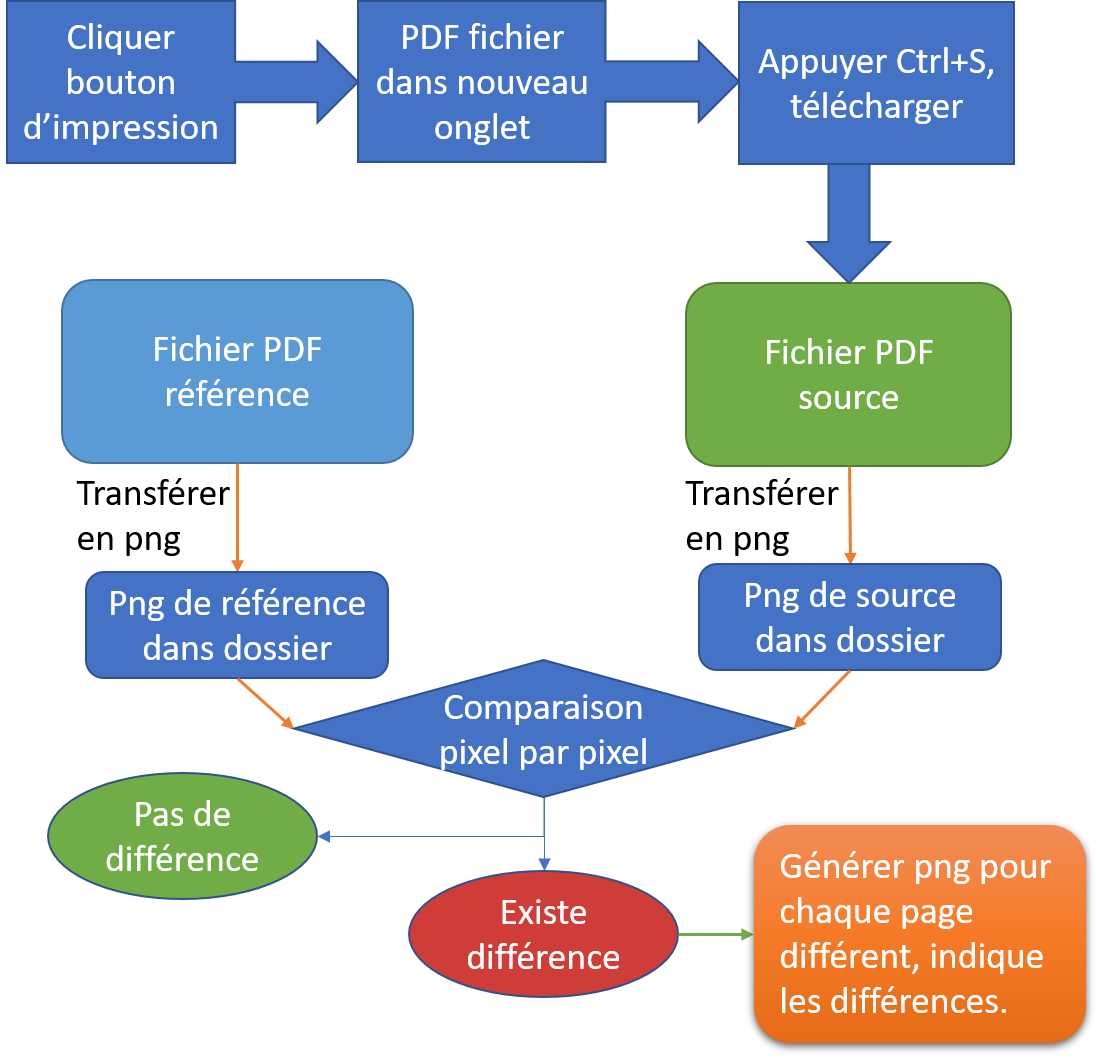
\includegraphics[width=8cm]{process_compar_pdf.png}
            \column{0.3\textwidth}
            \textcolor{red}{\textbf{Résulat : \newline \newline}}
            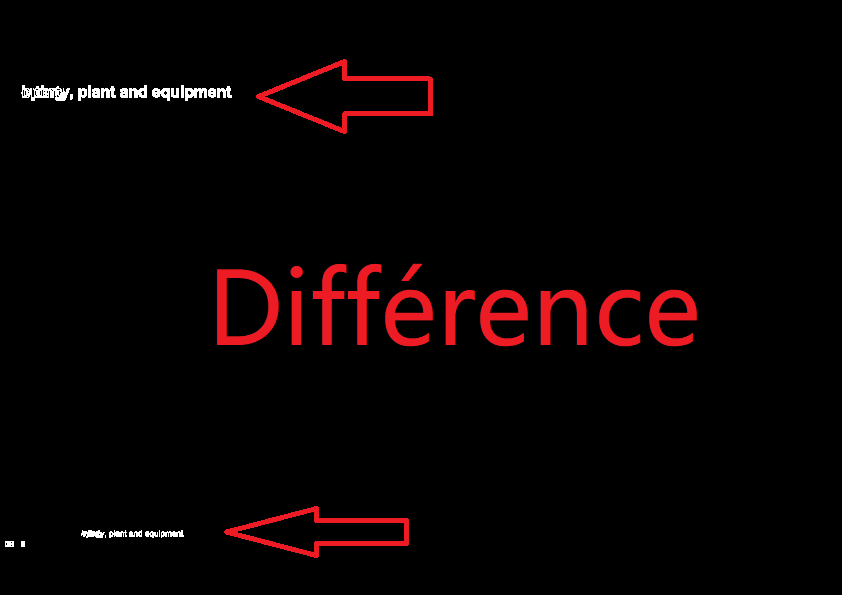
\includegraphics[width=\textwidth]{png_difference.png}
            \end{columns}
        \end{frame}
        
        %%%%%% Frame 14 %%%%%%
        \begin{frame}
        \frametitle{2\textsuperscript{ème} tâche: Téléchargement de zip, unzip, comparaison de PDF à la fin}
            \begin{block}{Problématique}
                \begin{itemize}
                    \item Pour cer tains scénario de tests, ils demandent FC télécharge un zip
                    \item Le nom de ce zip contient un GUID\textit{(globally unique identifier)} suffixe. 
                    \item Ce zip contient un nombre connu des fichiers en pdf avec le même GUID comme préfixe. Les noms des fichiers après décompression sont déjà donnés en ordre de temps de création dans le scénarios.
                \end{itemize}
            \end{block}
            \pause
            \begin{block}{Solution}
                \begin{itemize}
                    \item Utiliser la bibliothèque \textit{java.util.zip.ZipEntry} et \textit{java.util.zip.ZipInputStream} afin de décompresser le zip
                    \item Trier les fichiers en temps de créations puis les renommer avec les noms donnés, ensuite faire la comparaison. Pour trier, j'utilise $\lambda$-Expression.
                \end{itemize}
            \end{block}
        \end{frame}
        
        \begin{frame}
            \frametitle{2\textsuperscript{ème} tâche: Comparaison entre deux répertoire avec $\lambda$}
            \begin{block}{Problématique}
                \begin{itemize}
                    \item La même demande de téléchargement du zip
                    \item Mais on ne sait pas le nom ou le préfixe de nom, ni le nombre des fichiers PDFs dans le zip.
                    \item Autrement dit, ça nous demande de comparer entre deux zip, ils ont le même nombre des PDFs, et ces PDFs ont les même noms.
                \end{itemize}
            \end{block}
            
            \pause
            \begin{block}{solution $\lambda$}
                \begin{enumerate}
                    \item Décompresser le zip téléchargé, garde comme répertoire de référence.
                    \item Parcourir le répertoire de référence et mettre tous les fichiers PDF dans une liste
                    \item Parcourir le répertoire de source, en prenant la liste des PDF de référence, trouver le PDF avec le même nom, ensuite faire la comparaison en appelant la fonction de comparaison PDF développé.
                \end{enumerate}
            \end{block}
        \end{frame}
        
        %%%%%% Frame 15 %%%%%%
        \begin{frame}[fragile] % fragile option est pour insérer les codes
            \begin{block}{Comparaison entre deux répertoire avec $\lambda$}
            \begin{lstlisting}
Path dirRef = Paths.get(refFolder);
Path dirSrc = Paths.get(srcFolder);
// filter the .pdf file
List<Path> listRefPath = Files.list(dirRef)
	.filter(f -> f.toString().endsWith(".pdf"))
	.collect(Collectors.toList());
for (int ii = 0; ii < listRefPath.size(); ii++){
	Path refPath = listRefPath.get(ii);
	Path srcPath = Files.list(dirSrc).filter(path ->
	    path.getFileName().equals(refPath.getFileName()))
	    .findFirst().get();
	comparePDF(refPath.toString(), srcPath.toString());
}
            \end{lstlisting}
            \end{block}
        \end{frame}
        
        \subsection{Outils et Technologies utilisés}
        %%%%%% Frame 16 %%%%%%
        \begin{frame}
        \frametitle{Outils et Technologies utilisés}
            \begin{table}[l]
                \centering
                \begin{tabular}{|l|c|c|c|}
                    \hline
                    IDE & 
\includegraphics[width=2cm]{Eclipse_logo.png} & & \\
                    \hline
                    Communication &  
\includegraphics[width=2cm]{Skype_for_Business_logo.png} & 
\includegraphics[width=2cm]{Outlook_logo.png} & \\
                    \hline
                    Partager & 
\includegraphics[width=2cm]{Perforce_Logo.jpg} & 
\includegraphics[width=2cm]{OneDriveLogo.png} & 
\includegraphics[width=2cm]{OneNoteLogo.png}\\
                    \hline
                    Outils \& Bibliothèque & 
\includegraphics[width=2cm]{junit-logo.png} & 
\includegraphics[width=2cm]{silktest_logo.png} & 
\includegraphics[width=2cm]{jenkins_logo.png} \\
                    \hline
                \end{tabular}
                \label{tab:my_label}
            \end{table}
        \end{frame}
        
    \section{Conclusion}
        %%%%%% Frame 17 %%%%%%
        \begin{frame}
            \begin{alertblock}{Résultats de travail}
                \begin{itemize}
                    \item Les scénarios de test de 1\textsuperscript{ère} tâches sont bien intégrés dans le projet
                    \item Le projet de test d'impression est bien intégré dans le projet et tourne bien sur le projet Test-auto
                    \item Les erreurs de test sont affichés dans les logs de test
                    \begin{enumerate}
                        \item L'image à gauche, "OK" veut dire que le test passe bien, "ERROR" veut dire que le test ne passe pas ou une différence dans le rapport
                        \item L'image à droite indique les détailles d'erreur, la différence de rapport.
                    \end{enumerate}
                \end{itemize}
            \end{alertblock}
            
            \begin{columns}
                \column{0.5\textwidth}
                \begin{figure}
                    \centering
                    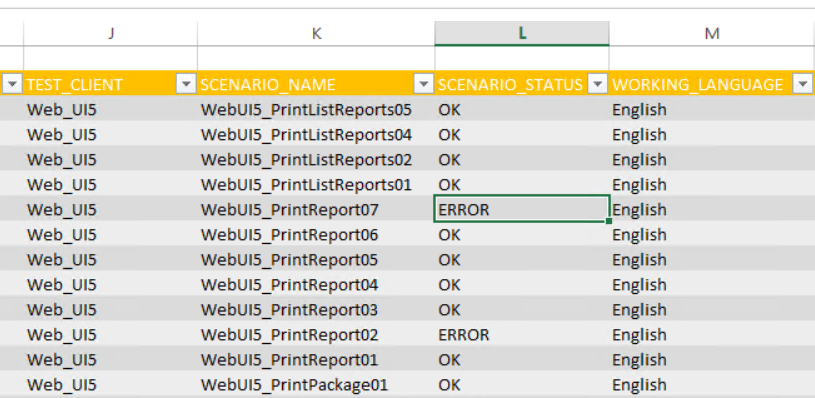
\includegraphics[height=2.4cm]{test_result.PNG}
                    \caption{Résultat de test}
                    \label{fig:result_test_label}
                \end{figure}
                
                \column{0.5\textwidth}
                \begin{figure}
                    \centering
                    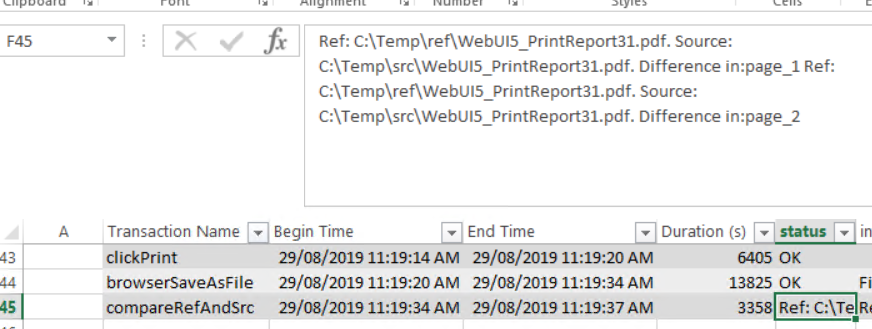
\includegraphics[height=2.2cm]{test_error_detail.PNG}
                    \caption{Détaille d'une erreur}
                    \label{fig:result_error_detail_label}
                \end{figure}
            \end{columns}
        \end{frame}
        
        %%%%%% Frame 18 %%%%%%
        \begin{frame}
            \begin{center}
                \LARGE{\textbf{Merci pour votre attention }} \textasciicircum\_\textasciicircum
            \end{center}
            
        \end{frame}
\end{document}